%%
%% This is file `sample-acmtog.tex',
%% generated with the docstrip utility.
%%
%% The original source files were:
%%
%% samples.dtx  (with options: `acmtog')
%% 
%% IMPORTANT NOTICE:
%% 
%% For the copyright see the source file.
%% 
%% Any modified versions of this file must be renamed
%% with new filenames distinct from sample-acmtog.tex.
%% 
%% For distribution of the original source see the terms
%% for copying and modification in the file samples.dtx.
%% 
%% This generated file may be distributed as long as the
%% original source files, as listed above, are part of the
%% same distribution. (The sources need not necessarily be
%% in the same archive or directory.)
%%
%% Commands for TeXCount
%TC:macro \cite [option:text,text]
%TC:macro \citep [option:text,text]
%TC:macro \citet [option:text,text]
%TC:envir table 0 1
%TC:envir table* 0 1
%TC:envir tabular [ignore] word
%TC:envir displaymath 0 word
%TC:envir math 0 word
%TC:envir comment 0 0
%%
%%
%% The first command in your LaTeX source must be the \documentclass command.
\documentclass[acmtog]{acmart}
\usepackage{graphicx}
\usepackage{caption}
\usepackage{subcaption}

\begin{document}

%%
%% The "title" command has an optional parameter,
%% allowing the author to define a "short title" to be used in page headers.
\title{CMIS Hand-in week 7}

%%
%% The "author" command and its associated commands are used to define
%% the authors and their affiliations.
%% Of note is the shared affiliation of the first two authors, and the
%% "authornote" and "authornotemark" commands
%% used to denote shared contribution to the research.
\author{Runfei Wu}
\email{qtx467@alumni.ku.dk}


%%
%% This command processes the author and affiliation and title
%% information and builds the first part of the formatted document.
\maketitle

\section{Idealization of a Dynamic Elastic Beam}
In this report, I will implement a 2D simulator to simulate dynamic hyper-elastic materials. The setup is we have a cantilever beam with the left boundary fixed to a rigid wall and the right boundary with some traction load. Last but not least, we have a gravity force acting on the beam. The beam is made of a hyper-elastic material, hence there will be elastic forces acting within the beam. The "dynamic" part is that the beam is moving with time as shown in Fig.~\ref{fig:setup}.
\begin{figure}[H]
    \centering
    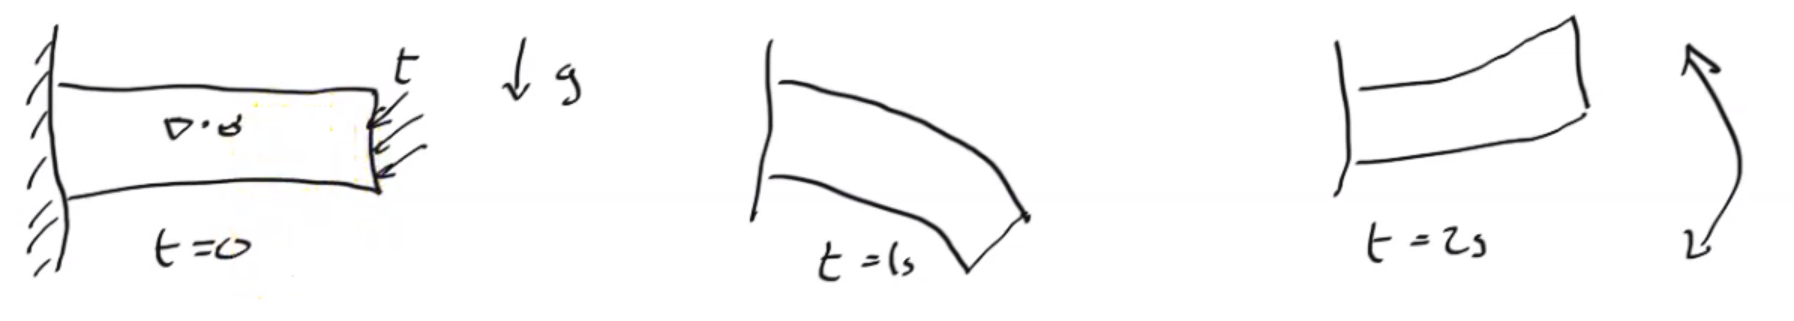
\includegraphics[width=0.9\linewidth]{images/setup.png}
    \caption{The setup of the simulation.}
    \label{fig:setup}
  \end{figure}
The simulation will start with the beam at rest position and the beam will deform with time. There will be no dissipation in the system, therefore, the total energy of the system should be conserved. Inside of the beam, the governing equation is the Cauchy equation. I choose a very specific version of the Cauchy equation, which is the Cauchy equation formulated with respect to the material coordinates. The reason for this choice is that the material coordinates are fixed with time, therefore, the computation will become much easier. 
Inside the beam, the governing equation is given by:
\begin{equation*}
\rho_0 \ddot{x} = b_0 + \nabla_X \cdot P
\end{equation*}
where $\rho_0$ is the density of the material, $b_0$ is the body force, $P$ is the first Piola-Kirchhoff stress tensor. On other boundary, we apply the Cauchy stress hypothesis as the boundary condition:
\begin{equation*}
    PN = t
\end{equation*}
where $N$ is the normal vector of the boundary given in the material coordinates and $t$ is the traction field. On the left boundary, we apply the Dirichlet boundary condition:
\begin{equation*}
    x = X_0
\end{equation*}
To set up the connection between the deformation and the stress inside the beam, we need a material model. In this report, I will use the Saint Venant-Kirchhoff model. The constitutive equation is given by:
\begin{equation*}
    S = \lambda tr(E)I + 2\mu E
\end{equation*}
where $S$ is the second Piola-Kirchhoff stress tensor, $\lambda$ and $\mu$ are the Lam\'e elasticity parameters, $E$ is the Green-Lagrange strain tensor. The Green-Lagrange strain tensor is given by:
\begin{equation*}
    E = \frac{1}{2}(F^TF - I)
\end{equation*}
where $F$ is the deformation gradient tensor. When we have computed the second Piola-Kirchhoff stress tensor, we can compute the first Piola-Kirchhoff stress tensor by:
\begin{equation*}
    P = F S
\end{equation*}
We will discuss how to compute the deformation gradient tensor when we get to the discretization part.

\section{Mesh}
In order to discuss the discretization of the governing equation, we need to first discuss the mesh. More specifically, we need to discuss the control volume type used in the finite volume method and the notation used. For the 2D mesh, I will use triangle mesh as the primary mesh and since I will use the finite volume method to discretize the governing equation, I will use the dual mesh as the computation mesh. The control volume type used is the median dual centered vertex control volume. The reason for this choice is that the median dual centered vertex control volume is a very simple control volume and it is very easy to compute the volume and the area of the control volume. It enables us to compute the flux across the boundary of the control volume very easily. The median dual centered vertex control volume is shown in Fig.~\ref{fig:mesh}.
\begin{figure}[H]
  \centering
  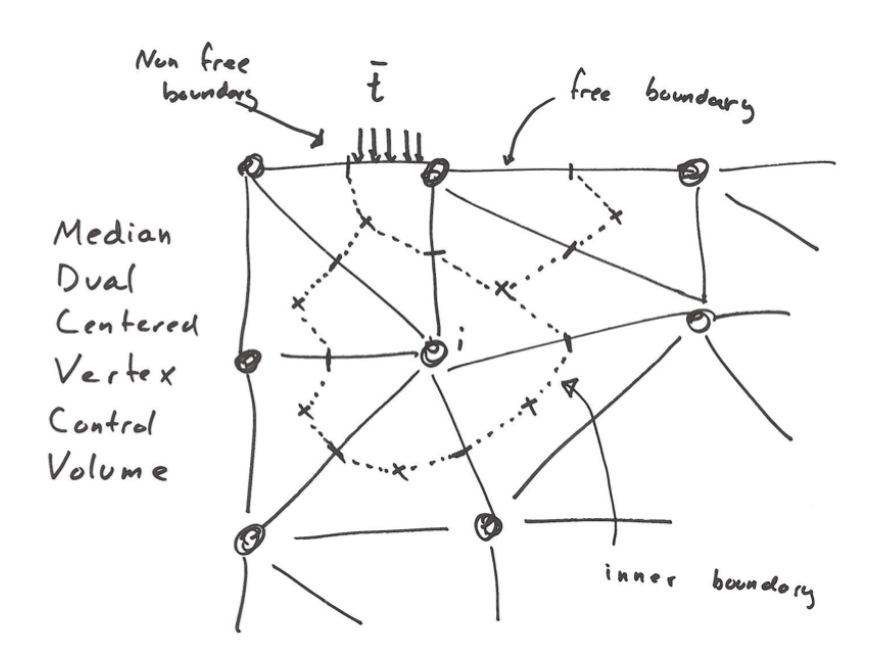
\includegraphics[width=0.9\linewidth]{images/mesh.png}
  \caption{The median dual mesh and the median dual centered vertex control volume.}
  \label{fig:mesh}
\end{figure}
The vertices of control volumes are defined by the barycenters of the triangles and the midpoints of the edges of the triangles. Every vertex of the primary mesh is the center of a control volume. The area of a control volume can be calculated by:
\begin{equation*}
    A = \sum_{t \in T(v)} \frac{1}{3}A_t
\end{equation*}
where $T(v)$ is the set of triangles that share the vertex $v$ and $A_t$ is the area of the triangle $t$. There are three types of boundaries in the mesh, the inner boundary which located inside the domain, and they are boundaries between control volumes. The free boundary which located on the boundary of the domain and there is no boundary condition applied. Finally, the non-free boundary which located on the boundary of the domain and there is boundary condition applied. For each control volume $i$, we denote the area $A_i$, within each triangle components, we denote the segments as $S_{ji}^e$, $S_{ki}^e$, $S_{\alpha}^e$, and $S_{\beta}^e$ as shown in Fig.~\ref{fig:cv}. 

\begin{figure}[htbp]
  \centering
  \begin{subfigure}[b]{0.235\textwidth}
       \centering
       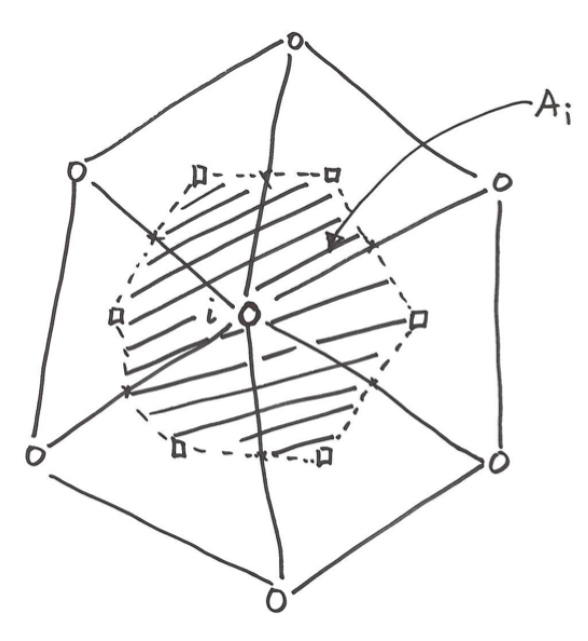
\includegraphics[width=\textwidth]{images/cv1.png}
       \caption{The control volume area.}
       \label{fig:cv1}
   \end{subfigure}
   \hfill
   \begin{subfigure}[b]{0.235\textwidth}
       \centering
       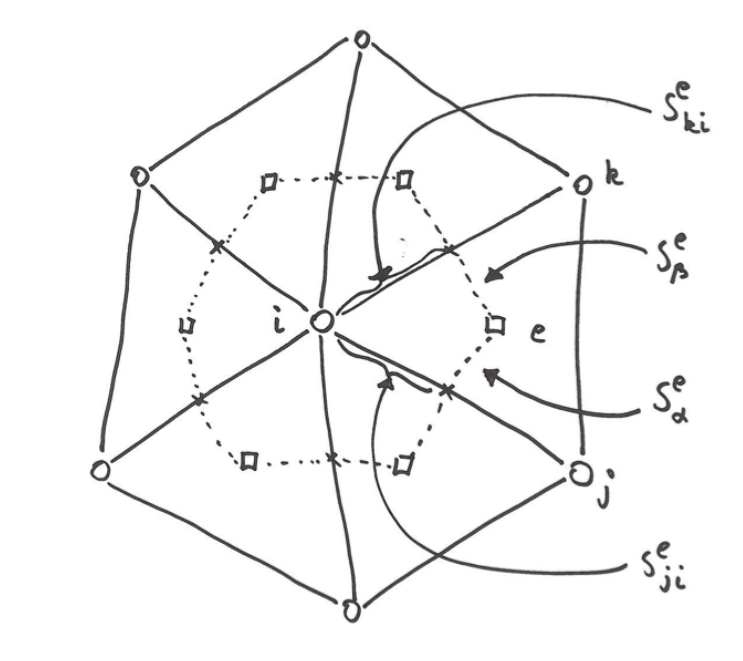
\includegraphics[width=\textwidth]{images/cv2.png}
       \caption{The control volume segments.}
       \label{fig:cv2}
   \end{subfigure}
  \caption{The control volume and the notation used.}
  \label{fig:cv}
\end{figure}

\section{Finite Volume Method on The Cauchy Equation}
Now that we have idealized the problem and the notation used to describe the mesh ready, we can start to discretize the governing equation.
\subsection{Discretization of The Cauchy Equation}
The first step of the finite volume method is to rewrite the governing equation in the volume integral form. The rewrite is given by:
\begin{equation*}
    \int_{v} \rho_0 \ddot{x} dv = \int_{v} b_0 dv + \int_{v} \nabla_X \cdot P dv
\end{equation*}
where $v$ is the volume of the control volume. Since we are working in 2D, therefore, volume in the above equation is actually the area. Then apply the Leibniz rule to the left-hand side of the equation, we get:
\begin{equation*}
    \frac{\partial^2}{\partial t^2} \int_{v} \rho_0 x dv = \int_{v} b_0 dv + \int_{v} \nabla_X \cdot P dv
\end{equation*}
Then we apply the midpoint approximation to the left-hand side of the equation, and we get:
\begin{equation*}
    \frac{\partial^2}{\partial t^2} \rho_0 A_i x_c = \int_{v} b_0 dv + \int_{v} \nabla_X \cdot P dv
\end{equation*}
where $x_c$ is the center coordinate of the control volume. Then we know that the $\rho_0A_i$ is the mass of the control volume, therefore, we can rewrite the equation as:
\begin{equation*}
    M_i \ddot{x}_c = \int_{v} b_0 dv + \int_{v} \nabla_X \cdot P dv
\end{equation*}
where $M_i$ is the mass of the control volume. Then we apply the midpoint approximation to the body force term, and we get:
\begin{equation*}
    M_i \ddot{x}_c = A_i b_0 + \int_{v} \nabla_X \cdot P dv
\end{equation*}
We can do this because the body force is constant in the control volume. One thing worth noting is that the mass inside a control volume is constant even though the mass density may change during the deformation. This is because we need to make sure the total mass of the beam is conserved. Then we apply the midpoint approximation to the divergence term, and we get:
\begin{align*}
    M_i \ddot{x}_c &= A_i b_0 + \int_{s_i} P \cdot \vec{n} ds \\
    &= A_i b_0 + \sum_{e} \sum_{\gamma \in \{\alpha, \beta\}} \int_{S_{\gamma}^e} P \cdot N ds
\end{align*}
where $s_i$ is the boundary of the control volume, $e$ is the related triangle component of the control volume, $\alpha$ and $\beta$ are the two edges of the triangle component, $N$ is the normal vector of the edge. We can start to simplify the equation, for the body force term we can replace it with $f_{ext, i}$ instead:
\begin{equation*}
  M_i \ddot{x}_c = f_{ext, i} + \sum_{e} \sum_{\gamma \in \{\alpha, \beta\}} \int_{S_{\gamma}^e} P \cdot N ds
\end{equation*}
Then we know for the free boundaries, the traction force is zero, therefore, $PN=t=0$. Then we can ignore the free boundaries, as they have no contribution to the integral. For the non-free boundaries where the traction force is not zero, we can replace the integral with the traction force $t$ instead:
\begin{equation*}
  \int_{S_{\gamma}^e} P \cdot N ds = \int_{S_{\gamma}^e} t ds=t l_{\gamma}^e
\end{equation*}
where $l_{\gamma}^e$ is the length of the edge. Then if we split the traction force out of the summation, we get:
\begin{align*}
  M_i \ddot{x}_c &= f_{ext, i} + \sum_{e} \left ( \sum_{\gamma1} l_{\gamma1}^e + \sum_{\gamma2} \int_{S_{\gamma2}^e} P \cdot N ds \right) \\
  &= f_{ext, i} + f_{t, i} + \sum_{e} \sum_{\gamma2} \int_{S_{\gamma2}^e} P \cdot N ds
\end{align*}
where $f_{t, i}$ is the traction force applied on the control volume $i$ and $\gamma1$ and $\gamma2$ are the edges where the traction force is not zero and zero respectively. Then we can further simplify the equation by midpoint approximation of the integral term. If we zoom into one triangle component as shown in Fig.~\ref{fig:zoom}.

\begin{figure}[H]
  \centering
  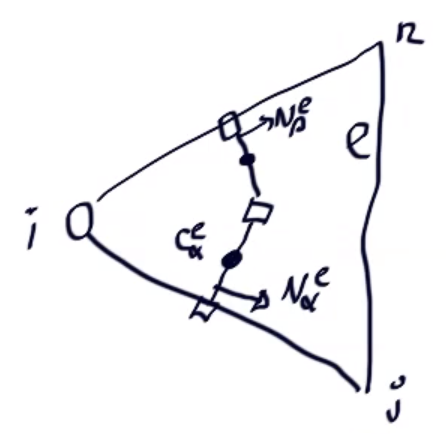
\includegraphics[width=0.35\textwidth]{images/zoom.png}
  \caption{Zoom into one triangle component.}
  \label{fig:zoom}
\end{figure}

we can see that the integral on the $S_{\alpha}^e$ and $S_{\beta}^e$ can be approximated by computing the stress tensor at the center of the edge and multiplying it with the outward normal vector of the edge. Then multiply the result by the length of the edge, and we get:
\begin{equation*}
  \int_{S_{\gamma2}^e} P \cdot N ds = P(c_{\gamma2}^e) \cdot N_{\gamma2}^e l_{\gamma2}^e
\end{equation*}
where $c_{\gamma2}^e$ is the center of the edge $\gamma2$ and $N_{\gamma2}^e$ is the outward normal vector of the edge $\gamma2$. At this point, we can see the advantage of the choice of using the Cauchy equation given in material coordinates. The outward normal vector of the edge and the length of the edge are all in the material coordinates which we can precompute before the simulation. The only thing we need to compute during the simulation is the stress tensor at the center of the edge. We will discuss how to compute the stress tensor at the center of the edge in the next section. 

\subsection{Computing The Deformation Gradient}
In order to compute the stress tensor at the center of the edge, we need to compute the deformation gradient. To define the deformation gradient, we need to define the deformation $\Phi$ first. The deformation $\Phi$ is a mapping from the material coordinates to the spatial coordinates as:
\begin{equation*}
  x = \Phi(X)
\end{equation*}
where $x$ is the spatial coordinates and $X$ is the material coordinates. Then the deformation gradient is essentially the derivative with respect to the material coordinates $X$ as:
\begin{equation*}
  F = \frac{x}{\partial X}=\frac{\partial \Phi}{\partial X}
\end{equation*}
We can also view the deformation gradient as a differentiable function from the material coordinates to the spatial coordinates: 
\begin{equation*}
  dx = F dX
\end{equation*}
where $dx$ is the differential of the spatial coordinates and $dX$ is the differential of the material coordinates. Then we can compute the deformation gradient by computing the differential of the spatial coordinates and the differential of the material coordinates. Specifically, when we compute the deformation gradient, we compute within each triangle component as shown in Fig.~\ref{fig:deformation}. 

\begin{figure}[H]
  \centering
  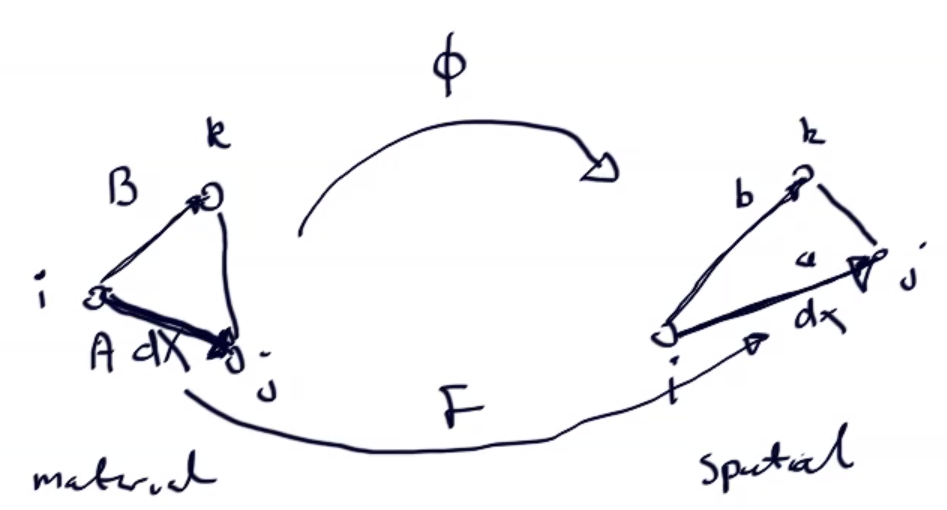
\includegraphics[width=0.5\textwidth]{images/deformation.png}
  \caption{Compute the deformation gradient within each triangle component.}
  \label{fig:deformation}
\end{figure}

from the center of the control volume $i$ we use the $ij$ and $ik$, the two edges of the triangle component, as the basis to compute the deformation gradient. In material coordinate, we mark the vector from $i$ to $j$ as $A$ and the vector from $i$ to $k$ as $B$. Then we mark the vector from $i$ to $j$ in the spatial coordinate as $a$ and the vector from $i$ to $k$ in the spatial coordinate as $b$. Then we can compute the deformation gradient using a linear system:
\begin{align*}
  a = F A \\
  b = F B 
\end{align*}
if we write the vectors in matrix form, we get:
\begin{equation*}
  \begin{bmatrix}
    a & b
  \end{bmatrix}
  =
  F
  \begin{bmatrix}
    A & B
  \end{bmatrix}
\end{equation*}
We denote the matrix $\begin{bmatrix} A & B \end{bmatrix}$ as $D_0^e$ and the matrix $\begin{bmatrix} a & b \end{bmatrix}$ as $D^e$. Then we can solve for the deformation gradient $F$ as:
\begin{equation*}
  F = D^e (D_0^e)^{-1}
\end{equation*}
where $(D_0^e)^{-1}$ is the inverse of the matrix $D_0^e$ and the good thing about this scheme is that as long as the triangle component is not degenerate, the matrix $D_0^e$ is invertible. So now we can compute the deformation gradient $F^e$ for each triangle component. Then we can use the deformation gradient $F^e$ to compute the Green-Lagrange strain tensor $E^e$ as:
\begin{equation*}
  E^e = \frac{1}{2} (F^e)^T F^e - I
\end{equation*}
where $I$ is the identity matrix. Then we can use the Green-Lagrange strain tensor $E^e$ to compute the second Piola-Kirchhoff stress tensor $S^e$ as:
\begin{equation*}
  S^e = \lambda tr(E^e) I + 2 \mu E^e
\end{equation*}
where $\lambda$ and $\mu$ are the Lame parameters. Then we can use the second Piola-Kirchhoff stress tensor $S^e$ to compute the stress tensor at the center of the edge $P^e$ as:
\begin{equation*}
  P^e = F^e S^e
\end{equation*}
Since we assume the deformation is linear within each triangle, then the deformation gradient $F^e$ is constant within each triangle component. Therefore, $E^e$, $S^e$ and $P^e$ are all constant within each triangle component. Now if we start to evaluate the integral:
\begin{equation*}
  \int_{S_{\gamma2}^e} P \cdot N ds = P(c_{\gamma2}^e) \cdot N_{\gamma2}^e l_{\gamma2}^e
\end{equation*}
because $P^e$ is constant within each triangle component, we do not need to compute $P(c_{\gamma2}^e)$ anymore. We can directly use the value of $P^e$ to calculate the elastic force at the edge $\gamma2$ as:
\begin{equation*}
  f_{\gamma2}^e = P^e N_{\gamma2}^e l_{\gamma2}^e
\end{equation*}

\subsection{The Clever Rewrite}
The main reason we use the median dual centered vertex control volume instead of the seemingly simpler dual edge control volume (shown in 
Fig.~\ref{fig:cv3}) is that it allows us to do a clever rewrite of the integral along the edges.

\begin{figure}[H]
  \centering
  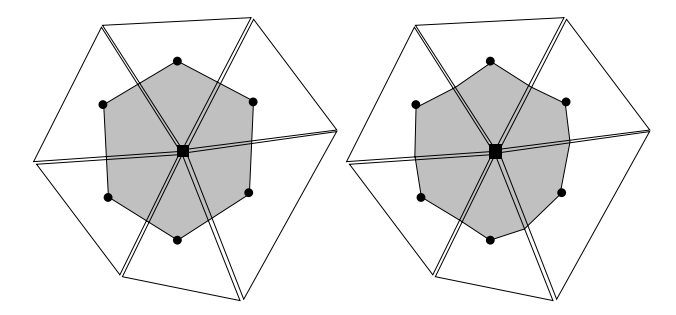
\includegraphics[width=0.5\textwidth]{images/cv3.png}
  \caption{The dual edge control volume (left), median dual centered vertex control volume (right).}
  \label{fig:cv3}
\end{figure}

One thing that will be very useful is the fact that if we have a closed surface integral of a constant vector field, then the integral is zero. Observe the integral:
\begin{equation*}
  \int_{S} P^e N^e ds
\end{equation*}
as we have discussed previously, $P^e$ is constant within each triangle component and $N^e$ is constant as it is defined in the material coordinate. Therefore, the integral is zero. This means that if we pick any closed surface within the mesh triangle, the integral will always be zero. Now we can pick the closed surface enclosed by the red and blue edges as shown in Fig.~\ref{fig:rewrite}.

\begin{figure}[H]
  \centering
  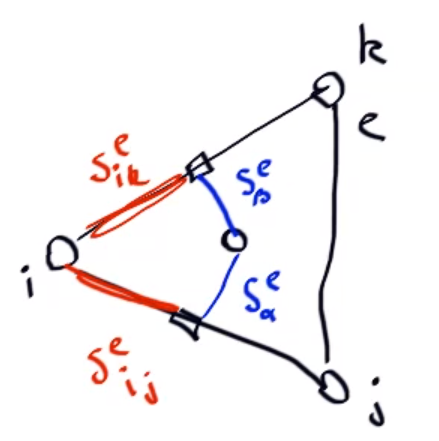
\includegraphics[width=0.35\textwidth]{images/rewrite.png}
  \caption{The closed surface we pick to rewrite the integral.}
  \label{fig:rewrite}
\end{figure}

We can expand the integral as:
\begin{equation*}
  \int_{S_{ij}^e} P^e N_{ij}^e ds + \int_{S_{ik}^e} P^e N_{ik}^e ds + \int_{S_{\alpha}^e} P^e N_{\alpha}^e ds + \int_{S_{\beta}^e} P^e N_{\beta}^e ds = 0
\end{equation*}

When we compute the elastic force at the edge $\gamma2$, we have to evaluate the integral along the $S_{\alpha}^e$ and $S_{\beta}^e$ edges. However, this can be hard to compute. But we can rewrite the integral as:
\begin{equation*}
  \int_{S_{\alpha}^e} P^e N_{\alpha}^e ds + \int_{S_{\beta}^e} P^e N_{\beta}^e ds = - \int_{S_{ij}^e} P^e N_{ij}^e ds - \int_{S_{ik}^e} P^e N_{ik}^e ds
\end{equation*}
and we can compute the integral along the $S_{ij}^e$ and $S_{ik}^e$ edges instead. More specifically, instead of computing the integral along the blue edges, we can compute the easier integral along the red edges. So now we can finally put everything together for our governing equation:
\begin{align*}
  M_i \ddot{x}_i &= f^{ext}_i + f^{t}_i + \sum_e \left ( \int_{S_{\alpha}^e} P^e N_{\alpha}^e ds + \int_{S_{\beta}^e} P^e N_{\beta}^e ds \right ) \\
  &= f^{ext}_i + f^{t}_i + \sum_e \left ( -\int_{S_{ij}^e} P^e N_{ij}^e ds - \int_{S_{ik}^e} P^e N_{ik}^e ds \right ) \\
  &= f^{ext}_i + f^{t}_i + \sum_e \left ( -\frac{1}{2}P^e N_{ij}^e l_{ij} - \frac{1}{2}P^e N_{ik}^e l_{ik} \right )
\end{align*}
where $l_{ij}$ and $l_{ik}$ are the length of the $S_{ij}^e$ and $S_{ik}^e$ edges respectively. If we rename the last term as $f^e_i$, we have a very compact form of the governing equation:
\begin{equation*}
  M_i \ddot{x}_i = f^{ext}_i + f^{t}_i + \sum_e f^e_i
\end{equation*}
and this is the final discretization of the governing equation we will use in our simulation.

\subsection{Time Discretization}
Now we have used FVM to do the spatial discretization of the governing equation, we just need to do the time discretization to complete our dynamic simulation. Previously, we have discretized the governing equation as:
\begin{equation*}
  M_i \ddot{x}_i = f^{ext}_i + f^{t}_i + \sum_e f^e_i
\end{equation*}
if we combine all the forces and rename them as $f^{total}_i$, we have:
\begin{equation*}
  M_i \ddot{x}_i = f^{total}_i
\end{equation*}
This is a second order ordinary differential equation. We can solve it by first rewriting it into two coupled first order ordinary differential equations:
we know that:
\begin{align*}
  \ddot{x} &=  \dot{v} \\
  v &= \dot{x} \\
\end{align*}
Therefore, we can rewrite the governing equation as:
\begin{equation}
  \label{eq:1}
  \dot{v}_i = \frac{1}{M_i} f^{total}_i
\end{equation}
\begin{equation}
  \label{eq:2}
  \dot{x}_i = v_i
\end{equation}
Then we use simple first order FDM to discretize the time derivative. More precisely, first order semi-implicit Euler time integration method. For the first equation, we have:
\begin{align*}
  \dot{v}_i &= \frac{v_i^{t+\Delta t} - v_i^t}{\Delta t}
\end{align*}
where $v_i^{t+\Delta t}$ is the velocity at time $t+\Delta t$ and $v_i^t$ is the velocity at time $t$. If we substitute the time derivative in Eq.~\ref{eq:1} with the discretized time derivative, we have:
\begin{equation*}
  v_i^{t+\Delta t} = v_i^t + \frac{\Delta t}{M_i} f^{total}_i
\end{equation*}
because we evaluate the velocity at time $t+\Delta t$ using the velocity at time $t$, this is an explicit part of the semi-implicit Euler method. For the second equation, we have:
\begin{equation*}
  \dot{x}_i &= \frac{x_i^{t+\Delta t} - x_i^t}{\Delta t}
\end{equation*}
where $x_i^{t+\Delta t}$ is the position at time $t+\Delta t$ and $x_i^t$ is the position at time $t$. If we substitute it into the Eq.~\ref{eq:2}, we have:
\begin{equation*}
  x_i^{t+\Delta t} = x_i^t + \Delta t v_i^{t+\Delta t}
\end{equation*}
notice we use the velocity at time $t+\Delta t$ to evaluate the position at time $t+\Delta t$, this is an implicit part of the semi-implicit Euler method. Now we have discretized the governing equation in both space and time, we can use it to simulate the dynamic behavior of the beam.

\subsection{Data Structure and associated Values} 
Now we have discretized the governing equation and all the notations ready, we can discuss a bit about the implementation of the simulation. For the primary triangle mesh, we will use two simple arrays, $T$ and $V$. $T$ is a $N \times 3$ array, where $N$ is the number of triangles in the mesh. Each row (element) of the array is a triplet of indices of the vertices that form a triangle. $V$ is a $M \times 2$ array, where $M$ is the number of vertices in the mesh. Each row (element) of the array is a pair of $x$ and $y$ coordinates of a vertex. In order to have easier access to the geometric information of the mesh, I will also have a class \texttt{MeshInfo} to store the geometric information of the mesh. Then for the computational mesh, I will use a class \texttt{VertexControlVolume} to store the information of each vertex control volume. The class will have the values for area, edge length, and edge outward unit normal etc., which will be used for those precomputed information. There will be three types of objects in our mesh, vertex, triangles, and edges. Each of them will have important data associated with them. For each vertex, the associated data will be the area of the corresponding control volume in material coordinates $A_i$, the material coordinates $X_i$, the spacial coordinates $x_i$, the spacial velocity $v_i$, and the total force applied to the corresponding control volume $f_i$. For the triangles, the associated data will be the deformation gradient $F^e$, the Green-Lagrange strain tensor $E^e$, the second Piola-Kirchhoff stress tensor $S^e$, the first Piola-Kirchhoff stress tensor $P^e$, and the $D^e_0$ matrix. For the edges, the associated data will be the edge length $l$, the edge outward unit normal $N^e$. The illustration for where we store the data is shown in Fig.~\ref{fig:data}.

\begin{figure}[h]
  \centering
  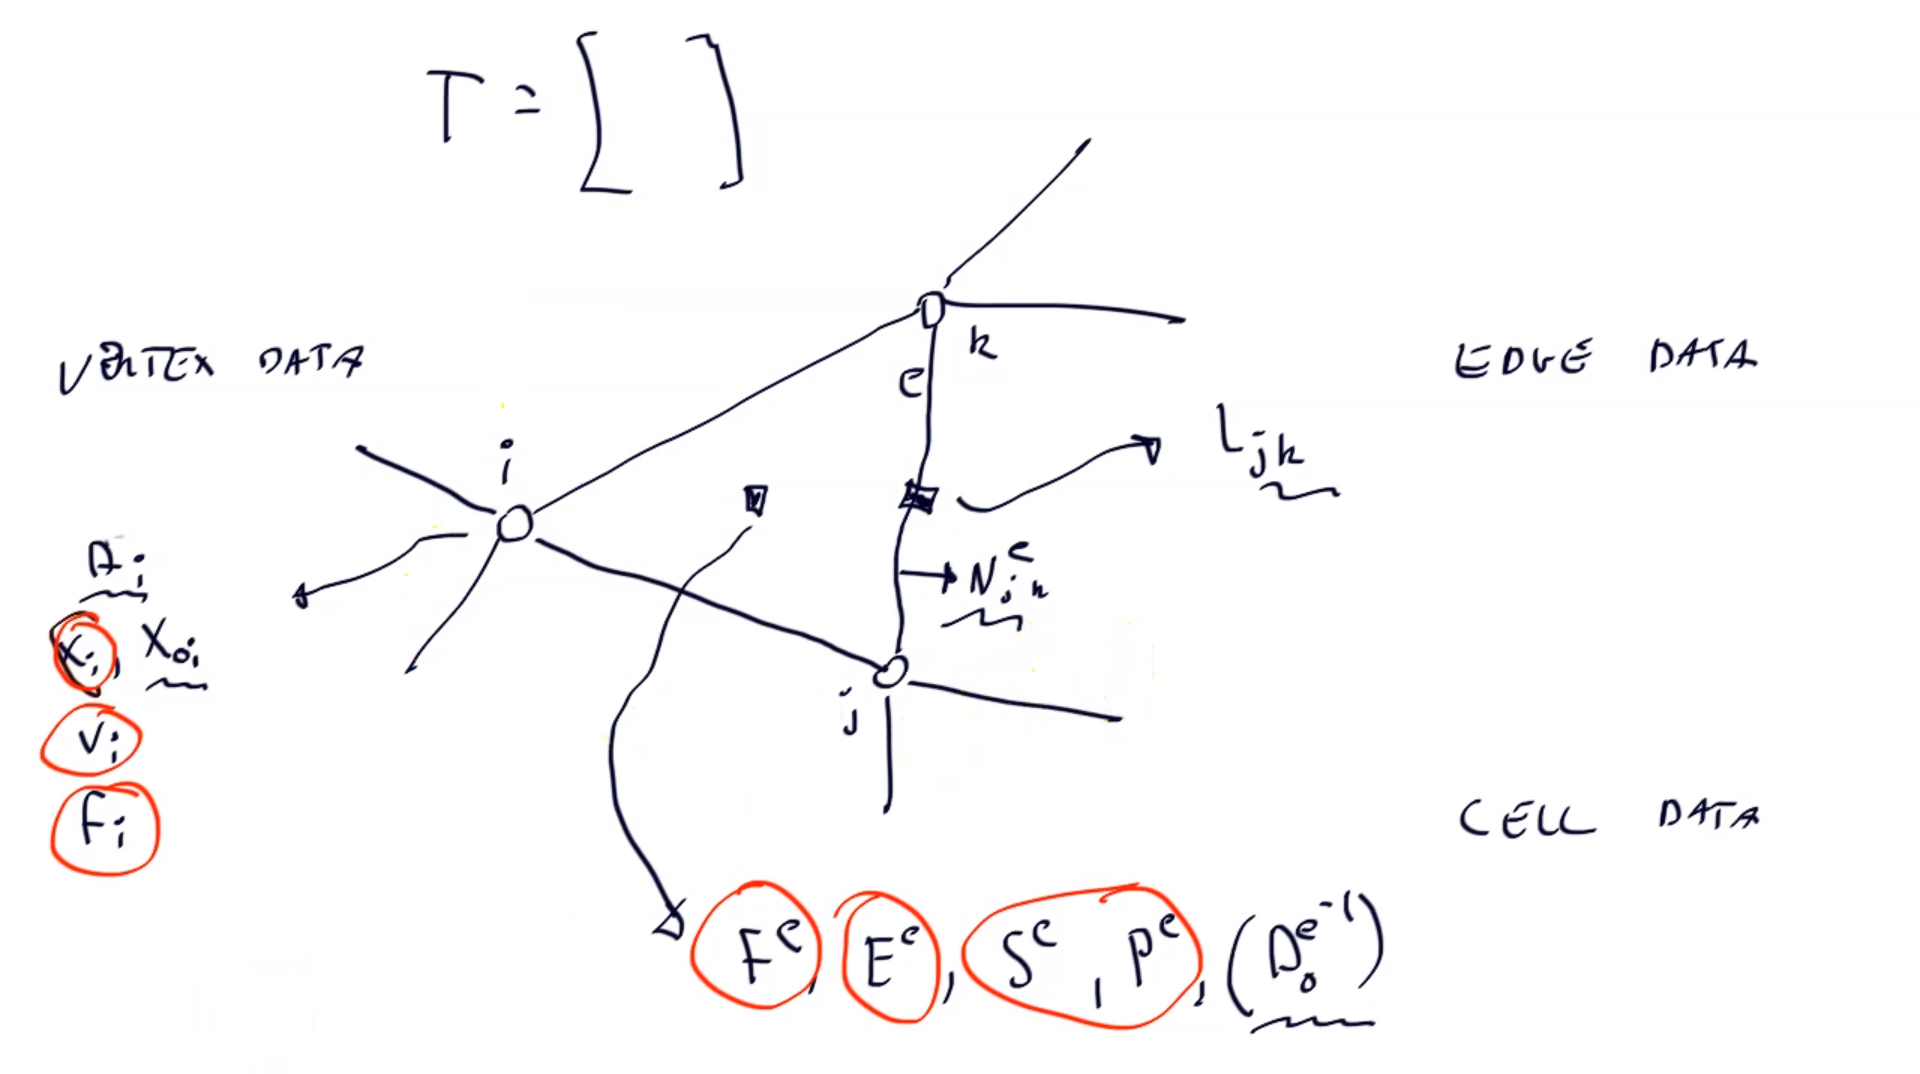
\includegraphics[width=0.5\textwidth]{images/data.png}
  \caption{Illustration of where the data is stored.}
  \label{fig:data}
\end{figure}

In the illustration, all the data that can be precomputed are underlined with wavy lines. All the data that need to be computed during the simulation are circled in red. Now we have everything sorted out, we can implement the simulation.

\section{Verification}
I implemented the simulation as described in the previous sections. In order to verify the correctness of the simulation, I first tested the simulation with a simple case where the beam is only under the gravity force. The beam is fixed at the left end and free at the right end. For the material parameters, Young's modulus, Poisson's ratio, and the mass density are set to be $E = 10^5$, $\nu = 0.3$, and $\rho = 100$. For the simulation parameters, the time step size is set to be $\Delta t = 0.001$. The simulation result at time $t=0$ is shown in Fig.~\ref{fig:gravity1}. 

\begin{figure}[H]
  \centering
  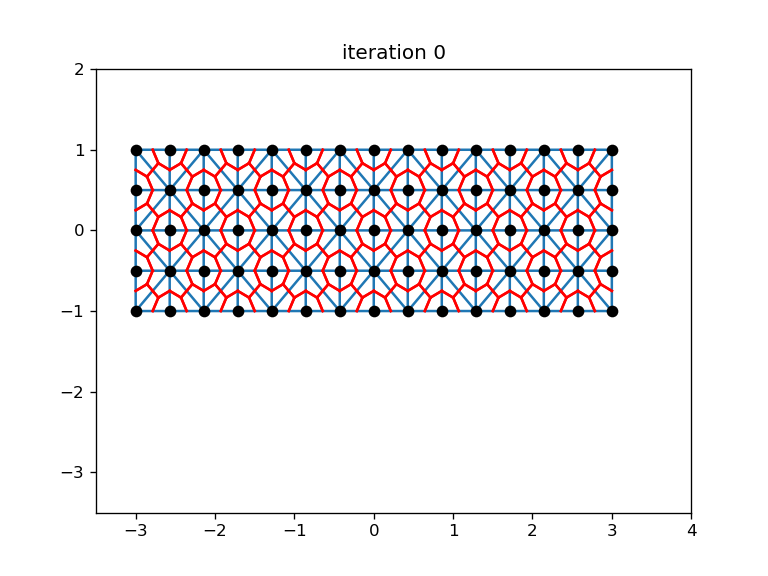
\includegraphics[width=0.5\textwidth]{images/gravity1.png}
  \caption{Simulation result at time $t=0$.}
  \label{fig:gravity1}
\end{figure}

This shows the initial state of the beam. The simulation result at time $t=200\Delta t$ is shown in Fig.~\ref{fig:gravity2}.

\begin{figure}[H]
  \centering
  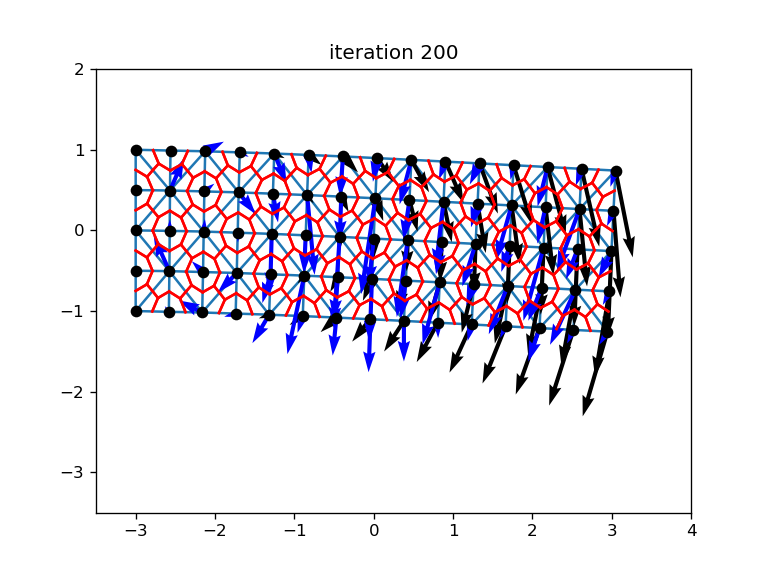
\includegraphics[width=0.5\textwidth]{images/gravity2.png}
  \caption{Simulation result at time $t=200\Delta t$.}
  \label{fig:gravity2}
\end{figure}

This shows the state of the beam after 200 time steps. All the black arrows show the velocity of the vertices. All the blue arrows show the total force applied to the vertices. You can see that because of gravity, the beam is bending downwards. The total force applied to each vertex and the velocity are pointing downwards. It is also worth noticing that the vertices which are closer to the fixed end have the force arrows pointing in a clockwise rotation. This is because the beam is fixed at the left end, so the vertex that is closer to the fixed end and near the top of the beam is actually being stretched and the vertex that is closer to the fixed end and near the bottom of the beam is actually being compressed forming a clockwise rotation with the force arrows. If we observe this rotation carefully, we can see that the rotation is actually moving inside the beam simulating the force propagation. The simulation result at time $t=500\Delta t$ is shown in Fig.~\ref{fig:gravity3}.

\begin{figure}[H]
  \centering
  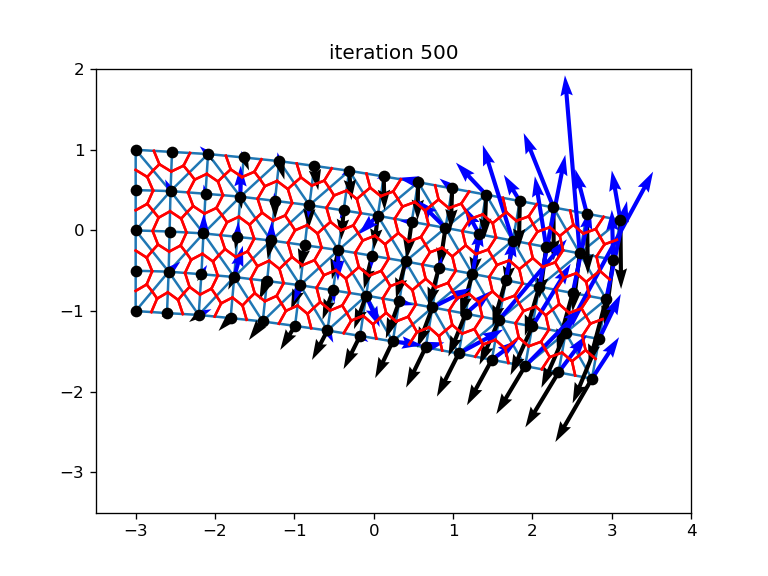
\includegraphics[width=0.5\textwidth]{images/gravity3.png}
  \caption{Simulation result at time $t=500\Delta t$.}
  \label{fig:gravity3}
\end{figure}

This shows the state of the beam after 500 time steps. You can see that the beam is still bending downwards. However, because the beam has passed the state where the internal elastic force is smaller than the gravity force, now the elastic force is actually pulling the beam upwards. But since the beam still has some kinetic energy, the velocity of the vertices is still pointing downwards. The simulation result at time $t=900\Delta t$ is shown in Fig.~\ref{fig:gravity4}.

\begin{figure}[H]
  \centering
  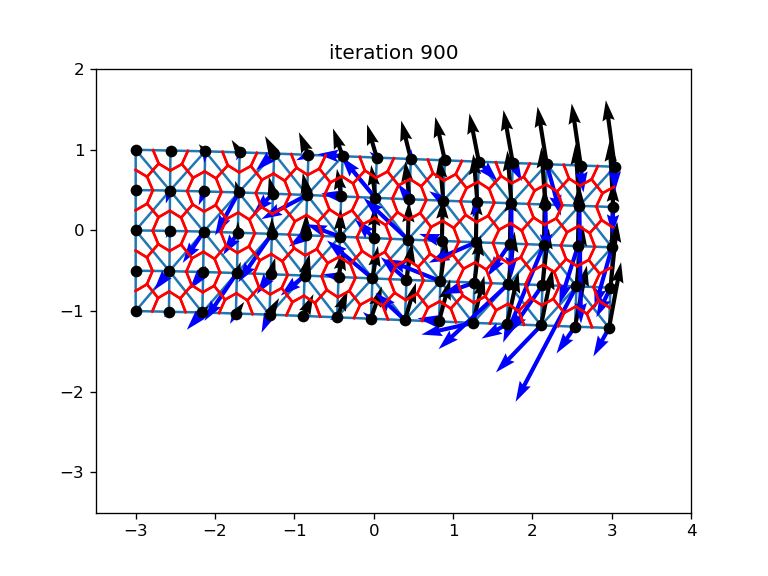
\includegraphics[width=0.5\textwidth]{images/gravity4.png}
  \caption{Simulation result at time $t=900\Delta t$.}
  \label{fig:gravity4}
\end{figure}

At this point the beam is bouncing up, however, since the beam is passed the equilibrium state where the gravity force is equal to the elastic force, the elastic force is now smaller than the gravity force, so all the blue arrows are pointing downwards but the velocity of the vertices are pointing upwards. Also because there is no dissipation in our simulation, the beam will keep bouncing up and down forever. So far the simulation result is consistent with our expectations. Now we can test the simulation with some different cases.

Before we start testing the simulation with different cases, we need to also check whether the traction force is correctly implemented or not. So I will apply a traction force to the right end of the beam and no gravity to keep things simple. The traction force is pointing downwards. The beam should band downwards. The result of the traction force is shown in Fig.~\ref{fig:base}.

\begin{figure}[H]
  \centering
  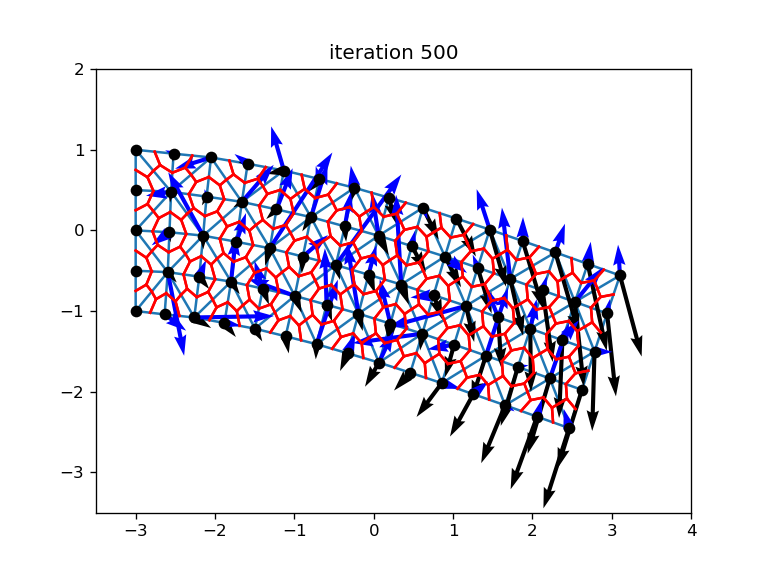
\includegraphics[width=0.5\textwidth]{images/base.png}
  \caption{Simulation result at time $t=500\Delta t$ with traction force.}
  \label{fig:base}
\end{figure}

You can see that the traction force is correctly implemented. The beam is indeed banding downwards as expected. We will use this as the base case for the following tests.

\subsection{Varing the Material Parameters}
If we carefully choose a material that is stiffer, the beam should bend less. In order to test this, this time we choose Yong's modulus to be $E = 1.5 \times 10^5$, and keep the other parameters and the setup the same as the base case. The simulation result at time step 500 of the new case is shown in Fig.~\ref{fig:material}.

\begin{figure}[H]
  \centering
  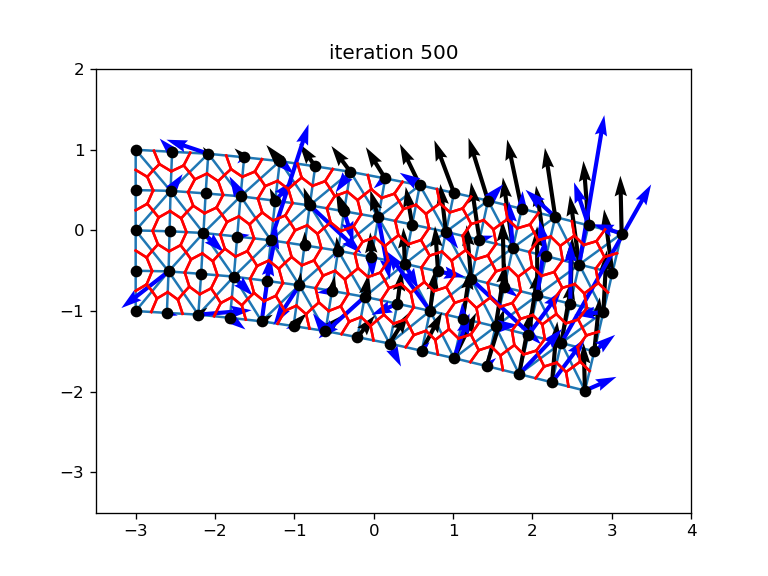
\includegraphics[width=0.5\textwidth]{images/material.png}
  \caption{Simulation result at time $t=500\Delta t$ with stiffer material.}
  \label{fig:material}
\end{figure}

You can see that the beam is bending less than the base case. You can easily tell this because the velocity of the vertices is already pointing upwards at time step 500 so the beam is starting to bounce back up whereas in the base case, the velocity of the vertices is still pointing downwards at time step 500 meaning the beam is still bending downwards. Besides, the bottom right tip of the beam has crossed the $y=-2$ line in the base case but it is not the case with the more stiff material. This is consistent with our expectations.

\subsection{Varying the Mesh Resolution}
If we increase the mesh resolution, the result should be more or less the same. In order to test this, this time we increase the mesh resolution from $14 \times 4$ to $18 \times 8$. The simulation result at time step 500 of the new case is shown in Fig.~\ref{fig:resolution}.

\begin{figure}[H]
  \centering
  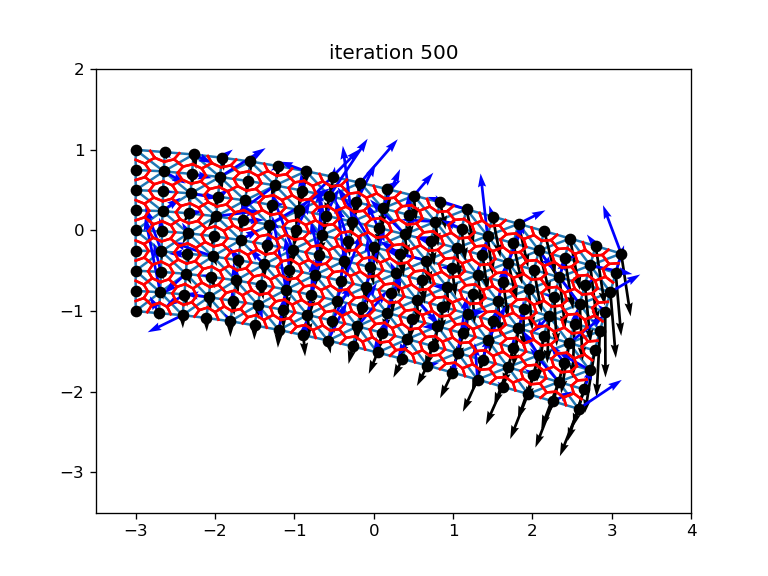
\includegraphics[width=0.5\textwidth]{images/resolution.png}
  \caption{Simulation result at time $t=500\Delta t$ with higher mesh resolution.}
  \label{fig:resolution}
\end{figure}

You can see that the beam is bending almost the same as the base case with some force pointing differently, but this may be due to the fact that we have more refined control volumes and the force is more accurately calculated. The coordinates and the velocity of the vertices are almost the same as in the base case. This is consistent with our expectations.

\subsection{Testing the Symmetry}
If we apply the traction force upwards instead of downwards, the beam should bend upwards. Since there is no gravity, the degree of the bending should be the same as the base case but the direction should be opposite. There should be a symmetry between the two cases. In order to test this, this time we apply the traction force upwards instead of downwards. The simulation result at time step 500 of the new case is shown in Fig.~\ref{fig:symmetry}.

\begin{figure}[H]
  \centering
  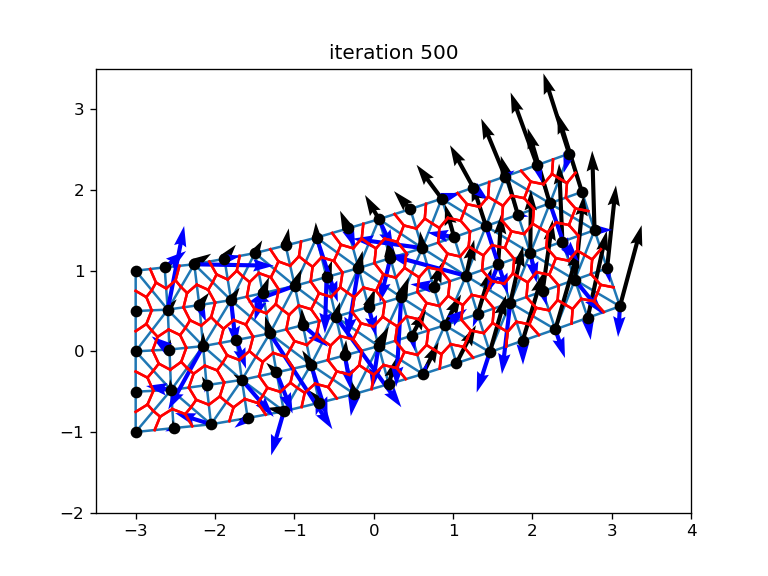
\includegraphics[width=0.5\textwidth]{images/symmetry.png}
  \caption{Simulation result at time $t=500\Delta t$ with traction force pointing upwards.}
  \label{fig:symmetry}
\end{figure}

You can see that the beam is bending upwards as expected.

\section{Validation}
After verifying that the simulation is working correctly, we can now validate the simulation by comparing the simulation result with the real world result. In order to do this, we need to find a real world example that can be modelled by our simulation. 
\subsection{Conservation of Energy}
In this project, we choose the law of conservation of energy as the validation example. The law of conservation of energy states that the total energy of an isolated system remains constant. In our simulation, we can easily calculate the total energy of the system at each time step. So we can compare the total energy of the system at different time steps to see if the total energy is conserved or not. If the total energy is conserved, then our simulation is validated. In order to do this, we need to first calculate the total energy of the system at each time step. The total energy of the system is the sum of the kinetic energy, the elastic energy and the gravitational potential energy.
\subsubsection{Only Horizontal Displacement}
To start things simple, we will first consider the case where the beam is only displaced horizontally. In this case, the gravitational potential energy is always zero. So the total energy of the system is the sum of the kinetic energy and the elastic energy. The kinetic energy is calculated by the following equation:
\begin{equation*}
E_k = \frac{1}{2} \sum_{i=1}^{N} m_i v_i^2
\end{equation*}
where $m_i$ is the mass of the $i$th control volume and $v_i$ is the velocity of the $i$th control volume. The elastic energy is a bit more complicated. The elastic energy is calculated by the following equation:
\begin{equation*}
E_{elas} = \sum_{i=1}^{N} \int_v \Psi(E(x)) dv
\end{equation*}
where $\Psi$ is the strain energy density function and $E(x)$ is the strain at position $x$. In our simulation, we use the following strain energy density function:
\begin{equation*}
\Psi(E) = \frac{1}{2} \lambda tr(E)^2 + \mu tr(E^2)
\end{equation*}
where $\lambda$ and $\mu$ are the Lame's parameters. The strain can be calculated during the simulation process. Then we know that the strain is constant in each triangle component, so we can write the elastic energy as:
\begin{equation*}
E_{elas} = \sum_{i=1}^{N} \sum_{e} \Psi(E^e) A_e
\end{equation*}
where $i$ is the index of the control volume, $e$ is the index of the triangle component, $E^e$ is the strain of the $e$th triangle component and $A_e$ is the area of the $e$th triangle component. So the total energy of the system is:
\begin{equation*}
E_{total} = E_k + E_{elas}
\end{equation*}

The way I set up the test is that I disabled the Dirichlet boundary condition and start the simulation with the beam in a horizontally compressed state. The beam was compressed by 10\% horizontally. The energy plot of the simulation is shown in Fig.~\ref{fig:godly}.

\begin{figure}[H]
  \centering
  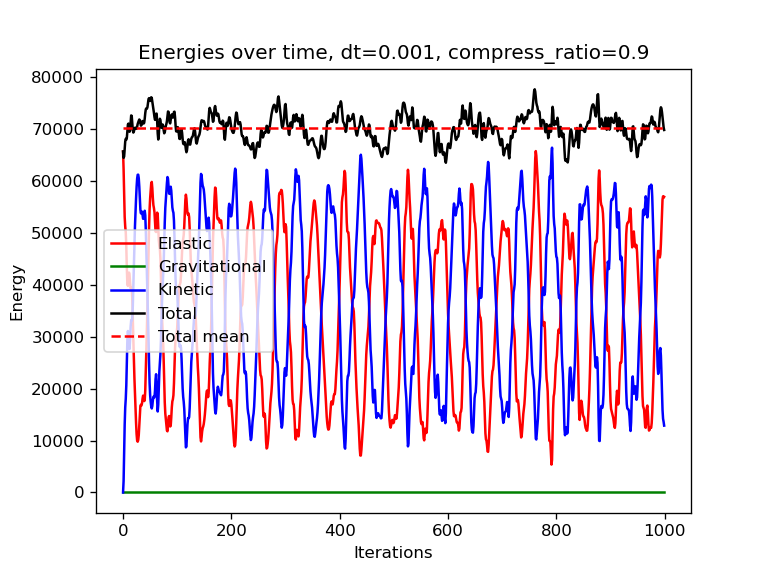
\includegraphics[width=0.5\textwidth]{images/godly.png}
  \caption{Energy plot of the simulation with only horizontal displacement.}
  \label{fig:godly}
\end{figure}

You can see that the gravitational potential energy is always zero. The kinetic energy and the elastic energy are oscillating around a certain value. I also plotted the total energy of the system in black, which is apparently not constant over time. This is because the simulation is not perfect. There are some numerical errors in the simulation. However, the total energy of the system is oscillating around a certain value. More precisely, the total energy of the system is oscillating around the mean which I plotted in orange. I can also show the error will decrease as we have more refined mesh and smaller time steps. The energy plot of the simulation with a more refined mesh and smaller time step is shown in Fig.~\ref{fig:godly2}.

\begin{figure}[H]
  \centering
  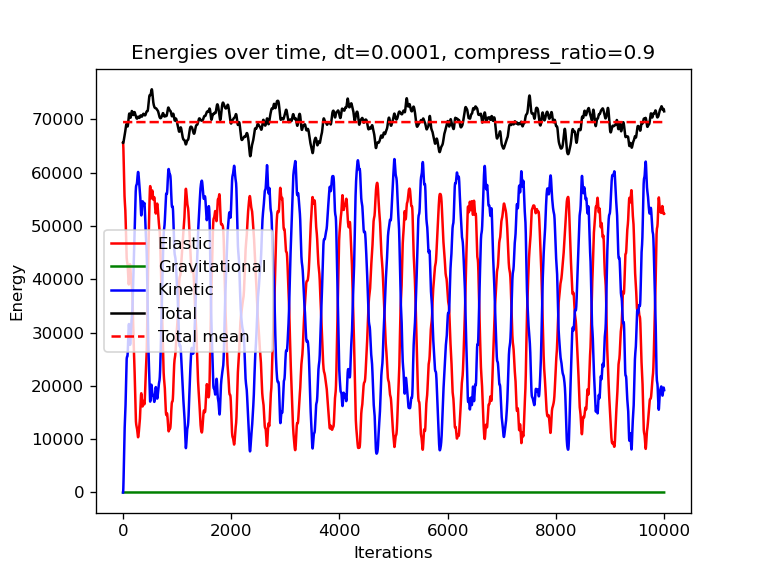
\includegraphics[width=0.5\textwidth]{images/godly2.png}
  \caption{Energy plot of the simulation with only horizontal displacement and more refined mesh.}
  \label{fig:godly2}
\end{figure}

In this graph, the fluctuation of the total energy of the system is significantly smaller. Therefore, we can conclude that the error is related to the mesh size and the time step. If we have a very refined mesh and a very small time step, the error will be very small. So we can say that the total energy of the system is conserved in our simulation.

\subsubsection{With External Force}
Now we will consider the case where we have applied the traction force on the right boundary for a certain period of time and the left boundary fixed to the wall. In this case, the gravitational potential energy will not be zero. So the total energy of the system is the sum of the kinetic energy, the elastic energy and the gravitational potential energy. The gravitational potential energy is calculated by the following equation:
\begin{equation*}
E_g = \sum_{i=1}^{N} m_i g \Delta y_i
\end{equation*}
where $m_i$ is the mass of the $i$th control volume, $g$ is the gravitational acceleration and $\Delta y_i$ is the vertical displacement of the $i$th control volume. So the total energy of the system is:
\begin{equation*}
E_{total} = E_k + E_{elas} + E_g
\end{equation*}
In this case, since there will be traction applied to the system, the total energy of the system will not be conserved at the beginning. However, after the traction is removed, the total energy of the system will be conserved. The energy plot of the simulation is shown in Fig.~\ref{fig:release}.

\begin{figure}[H]
  \centering
  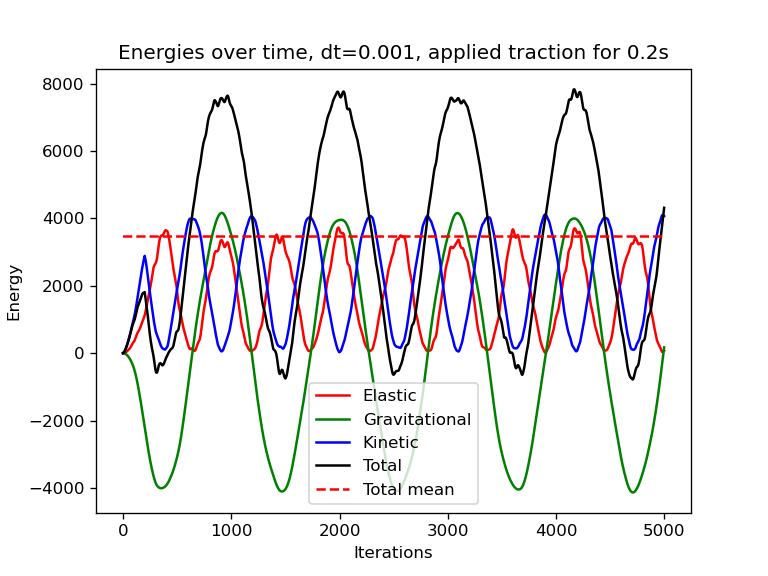
\includegraphics[width=0.5\textwidth]{images/release.png}
  \caption{Energy plot of the simulation with traction force.}
  \label{fig:release}
\end{figure}

You can see that the total energy of the system is still oscillating around a certain value. And if we observe closely, the initial oscillation is smaller than the oscillation later in time. This is because the traction force is removed at $t=0.2s$. So the total energy of the system is conserved after $t=0.2s$. With the additional gravitational potential energy, the range of the oscillation of the total energy of the system is larger than the case without external force. However, the total energy of the system is still conserved in our simulation as it is oscillating around a certain value. Hence we can conclude that the total energy of the system is conserved in our simulation and our simulation is valid.

\section{Limitations of The Model}
Obviously, our model is not perfect. There are some limitations of our model. In this section, I will discuss the two main limitations of our model. Namely, the inverted triangles and the time discretization scheme used in our simulation.
\subsection{Inverted Triangles}
In our simulation, we have not specified what happened when deformation is too much. If we applied an unrealistically large force to the system, the triangle components will be inverted and the whole simulation will crash. Let us imagine we only have horizontal deformation and nothing else. The ratio of deformation we denoted as $a$, then our deformation gradient matrix will be:
\begin{equation*}
F = \begin{bmatrix}
a & 0 \\
0 & 1
\end{bmatrix}
\end{equation*}
and the strain will be:
\begin{equation*}
E = \frac{1}{2} (F^T F - I) = \begin{bmatrix}
\frac{1}{2} (a^2 - 1) & 0 \\
0 & 0
\end{bmatrix}
\end{equation*}
The second Piola-Kirchhoff stress will be:
\begin{equation*}
S = \lambda tr(E) I + 2 \mu E = \begin{bmatrix}
  (\mu + \frac{\lambda}{2}) (a^2 - 1) & 0 \\
  0 & \frac{\lambda}{2} (a^2 - 1)
\end{bmatrix}
\end{equation*}
The first Piola-Kirchhoff stress will be:
\begin{equation*}
P = F S = \begin{bmatrix}
  (\mu + \frac{\lambda}{2}) (a^3 - a) & 0 \\
  0 & \frac{\lambda}{2} (a^2 - 1)
\end{bmatrix}
\end{equation*}

and for the $\mu + \frac{\lambda}{2}$ and $\frac{\lambda}{2}$ they are both positive constants, we can name them as $\alpha$ and $\beta$ respectively. So the first entry of the first Piola-Kirchhoff stress will be $\alpha (a^3 - a)$. Then cubic equation $\alpha (a^3 - a) = 0$ will introduce a very strange phenomenon. If we plot out the function $\alpha (a^3 - a)$, we will get the result shown in Fig.~\ref{fig:cubic}.

\begin{figure}[H]
  \centering
  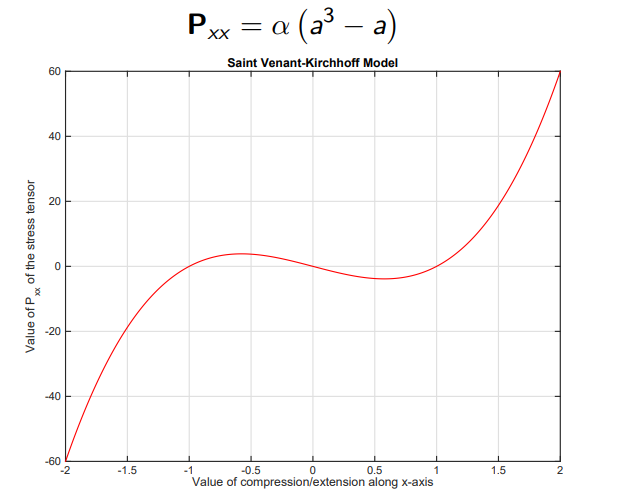
\includegraphics[width=0.30\textwidth]{images/cubic.png}
  \caption{Plot of the function $\alpha (a^3 - a)$.}
  \label{fig:cubic}
\end{figure}

We can see that at $a=1$, $a=-1$, and $a=0$, there is no stress response from the system. The most peculiar thing is that when $|a| < \frac{1}{\sqrt{3}}$ the material will stop resisting the compression and the stress response will gradually become zero around 0. This is when the model breaks. I also tested it in the simulator where I applied an unrealistically large horizontal force to the right boundary and fixed the left boundary to the wall. The last frame of the simulation before it crashes is shown in Fig.~\ref{fig:explode}.

\begin{figure}[H]
  \centering
  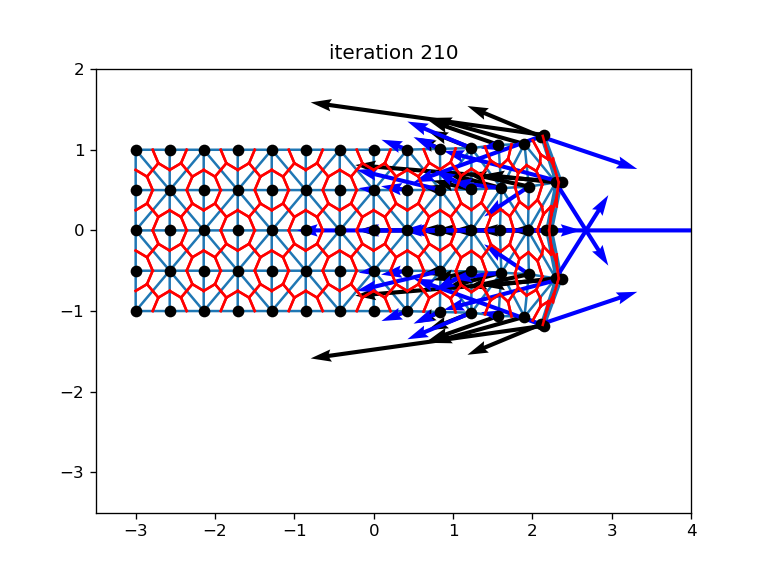
\includegraphics[width=0.40\textwidth]{images/explode.png}
  \caption{The last frame of the simulation before it crashes.}
  \label{fig:explode}
\end{figure}

As you can see that the triangles near the right boundary are almost crushed to a line. I have also plotted out the average elastic force of the system. The result is shown in Fig.~\ref{fig:explode2}.

\begin{figure}[H]
  \centering
  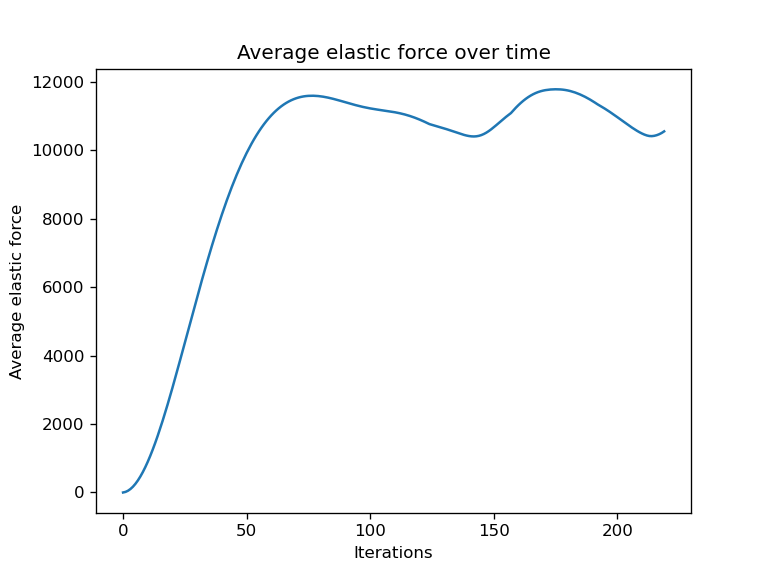
\includegraphics[width=0.35\textwidth]{images/explode2.png}
  \caption{The average elastic force of the system.}
  \label{fig:explode2}
\end{figure}

As you can see that the average elastic force of the system is not continuously increasing. At some point, the average force is actually decreasing which adheres to our analysis result previously.

\subsection{Time Discretization Scheme}
Another limitation is that in our simulation, we used the first order semi-implicit Euler time integration method to discretize the governing equation because it is simple and easy to implement. However, this method is not very accurate and it is not unconditionally stable. In our simulation, we used a very small time step to make sure the simulation is stable. However, this is not a good solution because it will increase the simulation time. Besides, as the time of the simulation increases, the error of the simulation will also increase. In the future, we can use a higher order time integration method to improve the accuracy and stability of the simulation.


\end{document}
\endinput
%%
%% End of file `sample-acmtog.tex'.
